\chapter{Initial Results}{\label{ch:Initial Results}
    \def\figpath{chapters/05/figures/}
    \graphicspath{ {\figpath} }

    \section{2-D Linear Source}{\label{sec:Results:2-D Linear Source}
        The \ac{LSMOC} method has been a significant part of this thesis work.
        The method, as described by \citet{Ferrer2016}, was implemented in MPACT \cite{Collins2016}, and has been significantly improved for cases with near-void regions \cite{Fitzgerald2018}, and multiphysics calculations \cite{Fitzgerald2019}.
        So far, detailed analysis has only been done for 2-D calculations; in this section, the results from a conference paper on the improved formulation are presented.
        Work done by others has indicated that for single physics (neutronics) calculations, significantly coarser meshes can be used with the \ac{LSA} as compared to the \ac{FSA} \cite{Ferrer2016,Boyd2014,Gunow2018}, resulting in faster computations; the goal of this conference paper was to present a reformulation of the method, that is more efficient in multi-physics calculations, as well as present results to indicate that coarser meshes could still be used \cite{Fitzgerald2019}.
        At the current time, all results are presented using \ac{TCP0} cross sections and odCMFD acceleration \cite{Zhu2016}.

        In this work, two additional physics are considered: isotopic depletion, and \ac{TH} feedback.
        Typical \acp{LWR} use \acs{UO2} fuel; however, a significant fraction of power comes from plutonium fission events.
        As a fuel rod is depleted during reactor operation, plutonium builds up in the outer rim of the fuel rods.
        In calculations with isotopic depletion, it is necessary to accurately capture this radial distribution of plutonium.
        In MPACT-CTF coupling, fuel temperatures are averaged radially.
        Since there is no radial dependence, it is not necessary to consider additional radial meshing to account for this physics.
        However, there is current work to add radially dependence to \ac{TH} feedback quantities in the coupling between MPACT and CTF, and this is common in other high fidelity neutronics codes.
        This may affect the number of rings needed in fuel meshes, for both the \ac{FSMOC} and \ac{LSMOC} solvers.

        To help determine optimal default meshing parameters for the \ac{LSMOC} solver in MPACT, a parametric study was done on a pin cell with isotopic depletion up to 70 MWD/kgHM.
        Using the default \ac{FSMOC} mesh as a starting point, the meshing parameters were coarsened; for each parameter, the coarsest option, that did not cause significant change in the eigenvalue over the depletion, was selected.
        The resulting coarse mesh has two fuel rings (inner radius at 87.5\% of outer), a single ring in the cladding, a single ring in the gap, and four azimuthal divisions in all regions.
        However, in the lattice and assembly test cases, a single azimuthal region was found to be sufficient in the fuel, clad, and gap material regions when using the \ac{LSMOC} solver.
        The inner fuel radius at 87.5\% of the outer radius is consistent with measured radial distributions of plutonium in irradiated \acs{UO2} fuel rods \cite{Lassmann1994}.
        This mesh, along with the default \ac{FSMOC} mesh, is shown in \cref{fig:Results:LSA:Depletion:Meshes}.

        Results from three cases are presented in the following subsections: 2D zero-power lattice cases, 2D lattice depletion cases, and a 3D fuel assembly with \ac{TH} feedback.

        \subsection{Pin Cell Isotopic Depletion}{\label{ssec:Results:LSA:Pin Cell}
            As reactors operate, interactions of the fuel with neutrons causes isotopic changes within the fuel, over long periods this can lead to significant changes in the fuel composition.
            Changes in the fuel composition play an important role in the power distribution as a reactor operates, and is thus a key additional physics to consider in reactor simulations.
            A parametric mesh-refinement study are presented for a single \acs{UO2} pin cell depletion up to 70 MWD/kgHM.

            During depletion, it is important to accurately capture the radial distribution of Plutonium due to self-shielding effects.
            However, Plutonium is primarily concentrated in the outer rim of the pin, this is the well known rim-effect.
            The expectation is that a single additional fuel ring can be used to capture this rim effect.
            This was found to be the case, with an inner ring with radius fraction 0.875 that of the outer fuel radius \cite{Fitzgerald2019}.
            This seems to be consistent with measured radial Plutonium distributions \cite{Lassmann1994}.
        }
        \subsection{2-D Zero-Power Lattice Cases}{\label{ssec:Results:LSA:2-D Zero-Power Lattice Cases}
            Initial tests were run on a series of zero-power 2-D lattices: the \ac{VERA} problem 2 cases \cite{VERAProblems}.
            By doing so, it can be verified that the \ac{LSMOC} solvers are as accurate on this coarse mesh as the \ac{FSMOC} solver on the current default mesh parameters in MPACT.
            These cases cover a variety of lattice configurations as different temperatures, with and without burnable absorbers or other inserts.
            Each case is described in detail in the reference \cite{VERAProblems}.

            Each lattice case was run with default and coarse meshes with the \ac{FSMOC} and \ac{LSMOC} solvers.
            Each of these cases used a Tabuchi-Yamamoto angular quadrature set \cite{TabuchiYamamotoQuad} with 64 azimuthal angles, 4 polar angles over 4$\pi$, and 0.05 cm ray-spacing.
            However, due to thin regions from IFBA and WABA rods in cases L, M, and N, a ray-spacing of 0.01 cm was used.
            The results are compared against a very finely meshed case run using the \ac{LSMOC} solver with 128 azimuthal angles, 4 polar angles, and 0.01 cm ray-spacing.
            Results are summarized in \cref{tab:Results:LSA:Zero Power Lattice Results}.

            On average, the \ac{LSMOC} solver on the coarse mesh is more accurate than the \ac{FSMOC} solver on the current default mesh.
            Additionally, the largest differences for both eigenvalue and RMS pin power differences are smaller than those for the \ac{FSMOC} solver.
            This indicates that, for these cases, the \ac{LSMOC} solver on the coarse mesh is sufficiently accurate.
            On average, the \ac{LSMOC} solver on the coarse mesh took 12\% less time per iteration, and used approximately 12\% less memory.

            \begin{table}[h]
                \centering
                \caption{Results for 2D zero-power lattice cases in terms of eigenvalue difference and RMS pin power difference from the very finely meshed \ac{LSMOC} solution.}
                \label{tab:Results:LSA:Zero Power Lattice Results}
                \begin{tabular}{rrrr@{\hskip 1cm}rrr}
                    \toprule
                    Case    & \multicolumn{3}{c}{$\Delta k_{\text{eff}}$ (pcm)} & \multicolumn{3}{c}{RMS Pin Power Difference (\%)}\\\midrule
                            & FS default   & FS coarse & LS coarse &  FS default   & FS coarse & LS coarse\\\midrule
                          A &    -17.37 &     43.98 &    -36.00 &      0.04 &      0.12 &      0.02\\
                          B &    -14.88 &     46.21 &    -33.83 &      0.04 &      0.12 &      0.02\\
                          C &    -17.37 &     43.98 &    -36.00 &      0.04 &      0.12 &      0.02\\
                          D &    -25.47 &     38.95 &    -40.97 &      0.04 &      0.12 &      0.02\\
                          E &    -49.02 &    -51.80 &    -26.93 &      0.06 &      0.18 &      0.02\\
                          F &    -74.17 &   -119.73 &    -25.68 &      0.05 &      0.18 &      0.02\\
                          G &    -98.35 &   -210.38 &    -42.52 &      0.08 &      0.26 &      0.04\\
                          H &    -77.90 &   -206.12 &     18.40 &      0.11 &      0.32 &      0.07\\
                          I &      2.36 &     82.42 &    -23.56 &      0.04 &      0.14 &      0.03\\
                          J &    -74.18 &   -119.45 &    -25.86 &      0.05 &      0.17 &      0.02\\
                          K &    -61.48 &    -97.41 &    -18.86 &      0.05 &      0.19 &      0.03\\
                          L &     60.38 &    104.64 &     52.02 &      0.06 &      0.17 &      0.05\\
                          M &     74.48 &    123.69 &     71.36 &      0.05 &      0.12 &      0.05\\
                          N &     -0.96 &    -44.92 &     42.85 &      0.11 &      0.32 &      0.04\\
                          O &    -21.26 &   -109.47 &      7.11 &      0.06 &      0.20 &      0.03\\
                          P &   -115.03 &   -311.33 &    -64.06 &      0.09 &      0.28 &      0.05\\
                          Q &    -12.26 &     53.68 &    -30.41 &      0.04 &      0.13 &      0.03\\\midrule
                        Avg. &     46.88 &    106.36 &     35.08 &      0.06 &      0.18 &      0.03\\
                        Max. &    115.03 &    311.33 &     71.36 &      0.11 &      0.32 &      0.07\\\bottomrule
                \end{tabular}
            \end{table}
        }
        \subsection{2-D Lattice Depletion}{\label{ssec:Results:LSA:2-D Lattice Depletion}
            In \cref{ssec:Results:LSA:2-D Zero-Power Lattice Cases}, the \ac{LSMOC} on the coarse mesh was shown to be sufficiently accurate for an array of lattice problems at zero-power.
            Two of these problems, 2a and 2p, were selected for further study by performing isotopic depletion up to 70 MWD/kgHM at HFP conditions.
            Problem 2A represents a typical lattice configuration consisting only of fuel rods and empty guide-tubes.
            Problem 2P contains several gadolinia rods that act as burnable absorbers; reactivity is significantly damped at beginning of cycle, but increases as gadolinia is burned.
            The gadolinia rods require significant radial meshing to accurately capture the complicated distribution throughout the depletion (it is an effectively a \emph{moving boundary layer}); the default meshing for the \ac{FSMOC} solver has 10 equal volume rings in the fuel.
            Due to this complicated distribution, the \ac{LSMOC} solver can only eliminate two of the additional radial rings while maintaining the same level of accuracy as the \ac{FSMOC} solver on the current default mesh.
            However, similar azimuthal coarsening is possible on these rods, with a single azimuthal region in all but the surrounding moderator, which has 4 azimuthal regions.
            Overall, a significant reduction in the lattice mesh is still possible, as shown in \cref{fig:Results:LSA:Depletion:Meshes}.

            As shown in \cref{fig:Results:LSA:Lattice Depletion Results}, the \ac{LSMOC} solver on a coarse mesh has similar accuracy as the \ac{FSMOC} solver on the current default mesh.
            However, the coarse mesh \ac{LSMOC} calculation took took 23\% and 18\% less time for cases A and P, respectively, than the corresponding default mesh \ac{FSMOC} calculations.
            Although the \ac{LSMOC} method was intended, primarily, to increase efficiency in the \ac{MOC} calculation, much of the time saved is actually from reduced time in the isotopic depletion routines.
            21\% and 18\% less memory was used by MPACT in cases A and P, respectively.
            \begin{figure}[h]
                \centering
                \begin{minipage}{0.25\linewidth}
                    \centering
                    \begin{subfigure}[t]{\linewidth}
                        \centering
                        
\includegraphics[width=0.45\linewidth]{\figpath/pin/pin-default.png}
                        \caption{Default fuel rod mesh\\\centering(56 cells)}
                    \end{subfigure}
                    \begin{subfigure}[t]{\linewidth}
                        \centering
                        
\includegraphics[width=0.45\linewidth]{\figpath/pin/pin-coarse.png}
                        \caption{Coarse fuel rod mesh\\\centering(20 cells)}
                    \end{subfigure}
                \end{minipage}%
                ~
                \begin{minipage}{0.75\linewidth}
                    \centering
                    \begin{subfigure}[t]{0.40\linewidth}
                        \centering
                        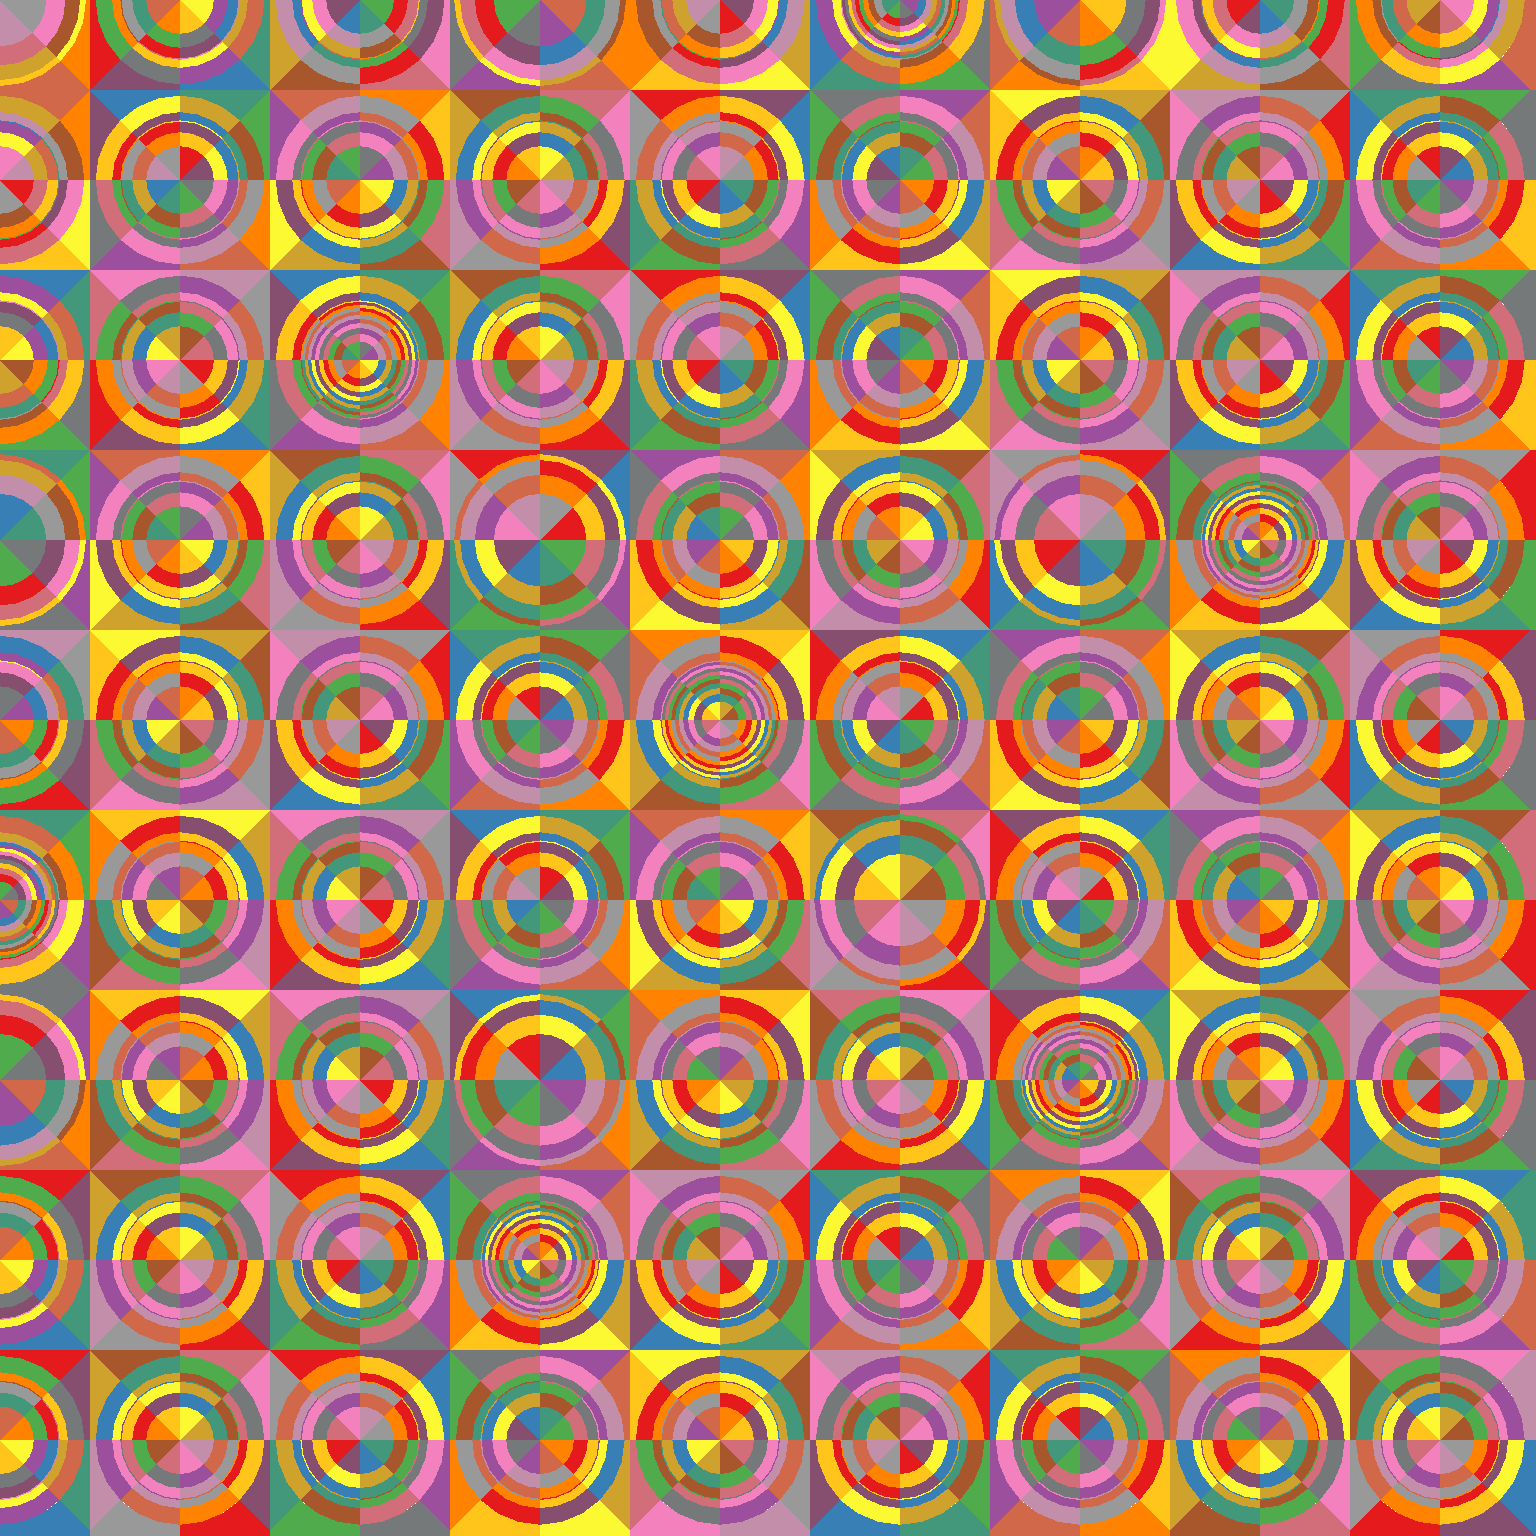
\includegraphics[width=\linewidth]{\figpath/lattice/2p/default.png}
                        \caption{Default lattice (2p) mesh\\\centering(4282 cells)}
                    \end{subfigure}%
                    ~
                    \begin{subfigure}[t]{0.40\linewidth}
                        \centering
                        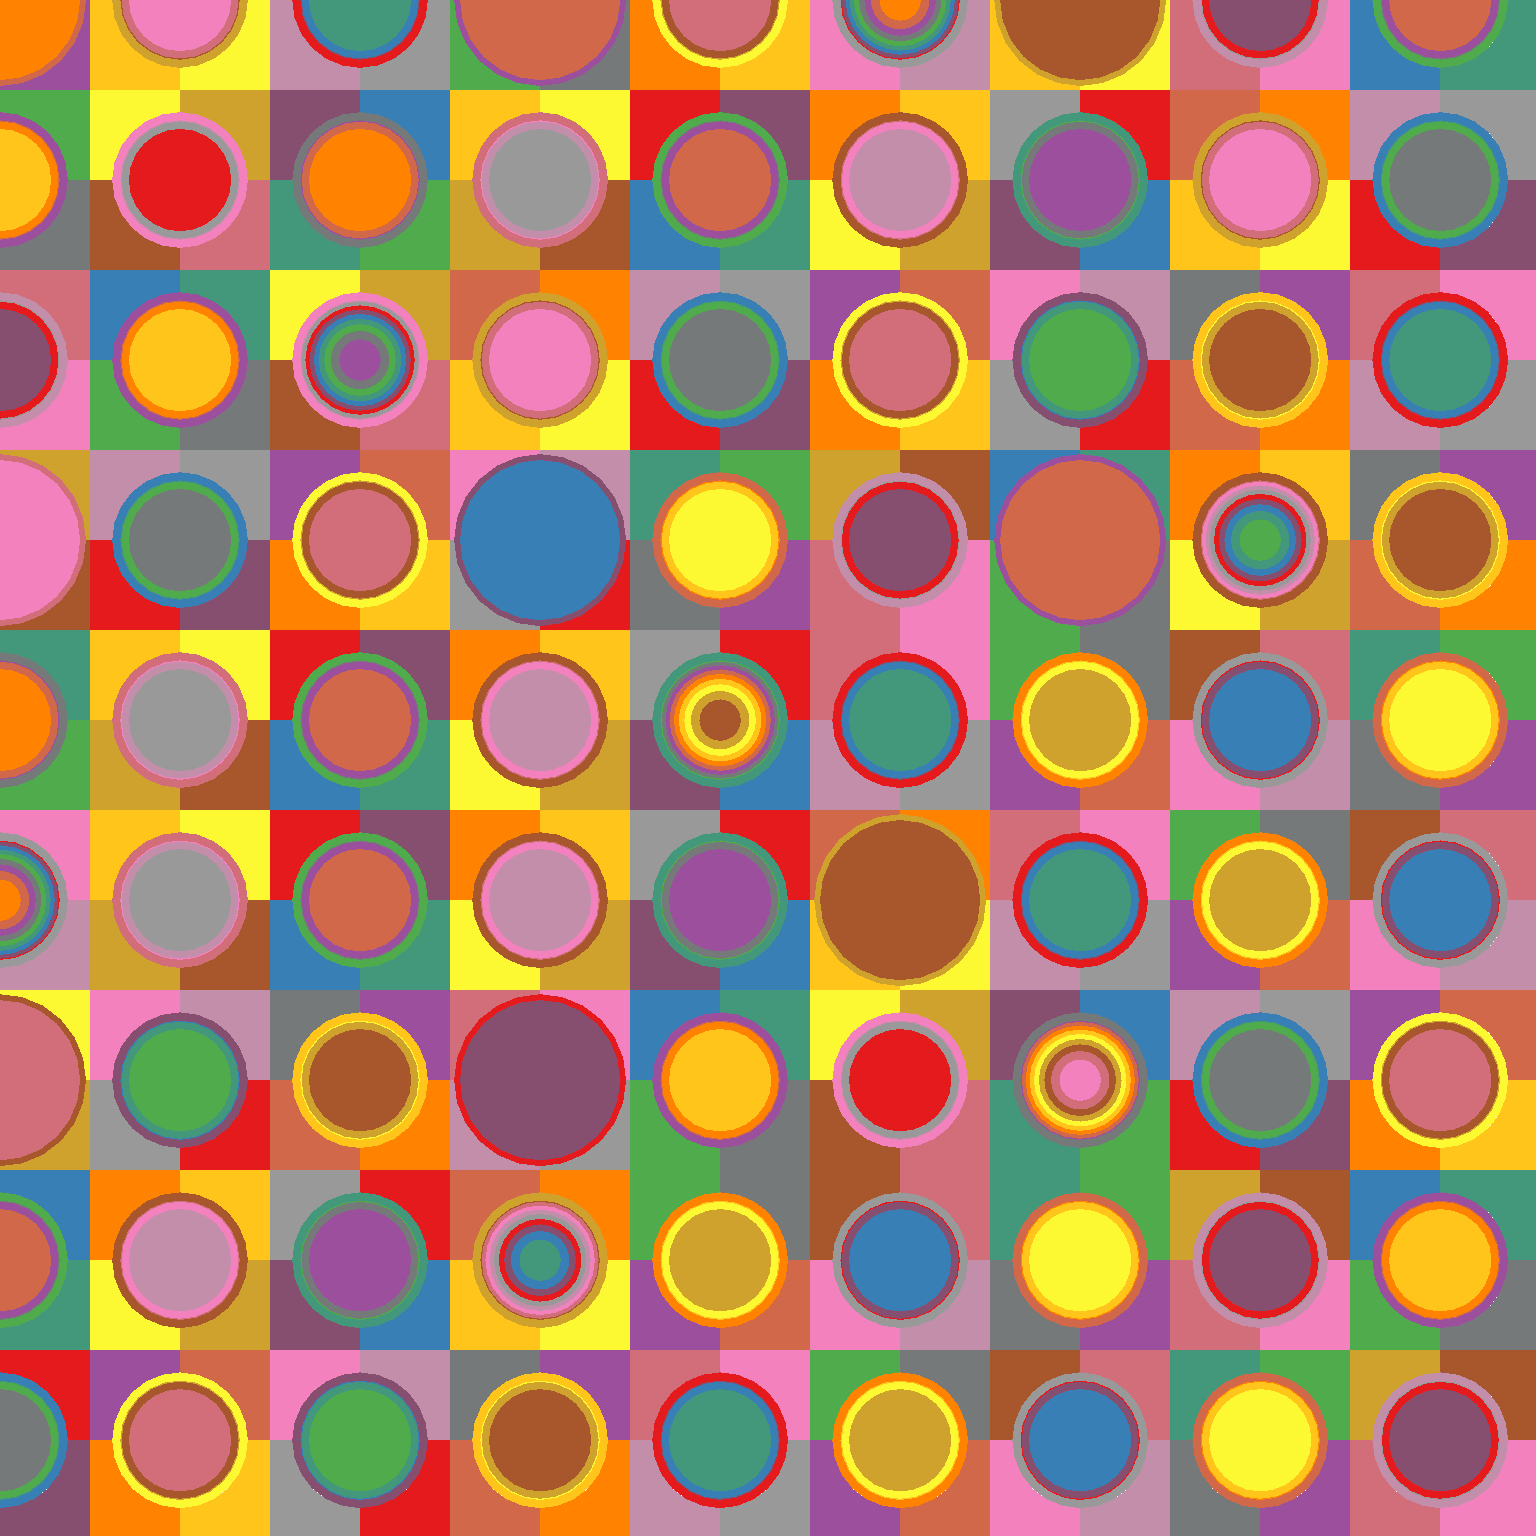
\includegraphics[width=\linewidth]{\figpath/lattice/2p/coarse.png}
                        \caption{Coarse lattice (2p) mesh\\\centering(637 cells)}
                    \end{subfigure}
                \end{minipage}
                \caption{Current default and coarse meshes for pin and lattice (2P) calculations.}
                \label{fig:Results:LSA:Depletion:Meshes}
            \end{figure}
            \begin{figure}[h]
                \centering
                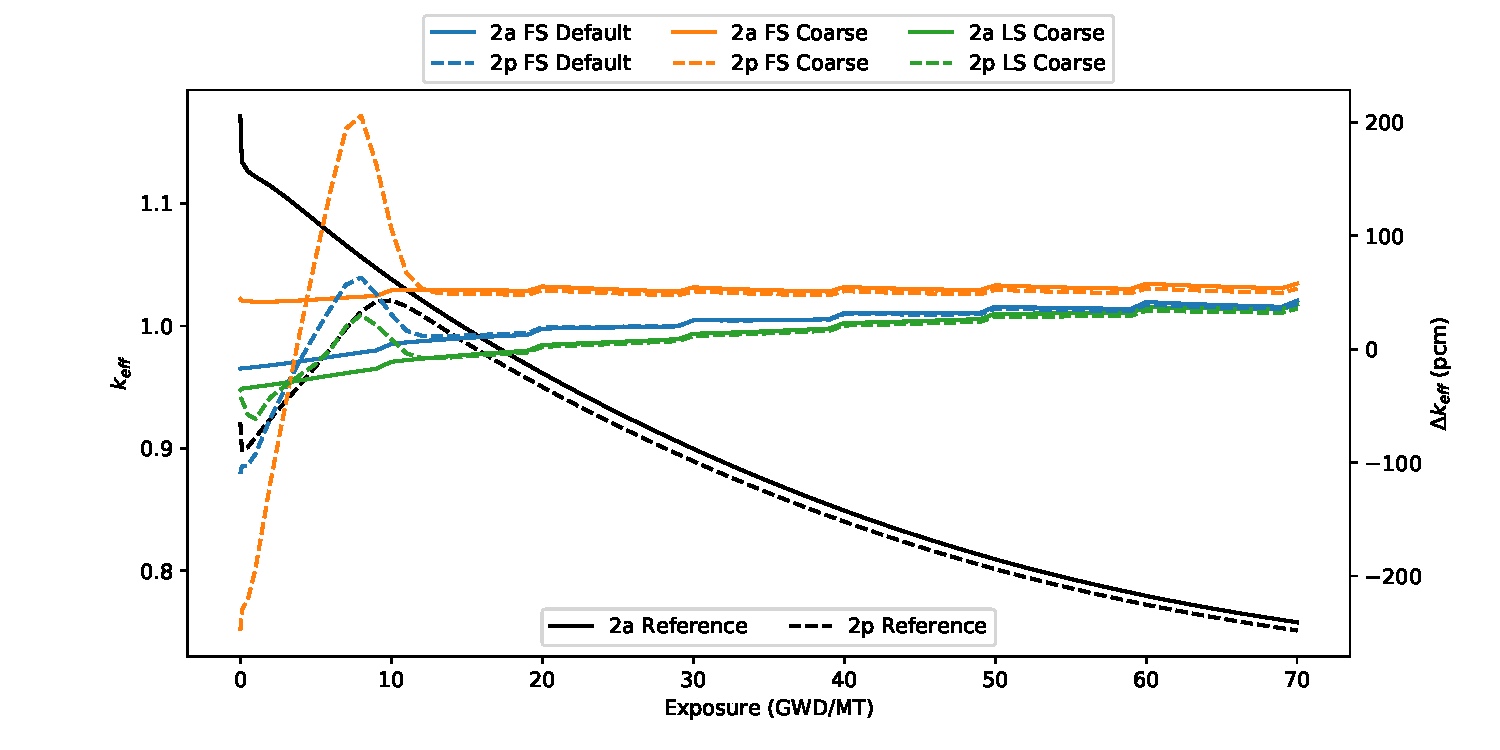
\includegraphics[width=0.85\linewidth]{\figpath/lattice/2p/lattice-depl-summary.pdf}
                \caption{Eigenvalue reference values and differences for default, and coarse mesh calculations throughout isotopic depletion of VERA problems 2A and 2P up to 70 MWD/kgHM.}
                \label{fig:Results:LSA:Lattice Depletion Results}
            \end{figure}
        }
        \subsection{3-D Assembly with T/H Feedback}{\label{ssec:Results:LSA:3D Assembly with T/H Feedback}
            The final case examined in this work was a single 3D assembly with \ac{TH} feedback: VERA problem 6 \cite{VERAProblems}.
            This case demonstrates that a coarser mesh can be used with the \ac{LSMOC} solver in problems with \ac{TH} feedback and in the 2D/1D framework \cite{Collins2016}.
            Meshing parameters from the previous results were used in fuel and guide-tube elements.
            The lower and upper plates and nozzles are meshed as rectilinear grids in MPACT; these were able to be coarsened to 0.42$\times$0.42 cm$^2$ sized elements.

            This case was run with the default and coarse meshes with the \ac{FSMOC} and \ac{LSMOC} solvers.
            Each calculation was compared against a finely meshed case run with the \ac{LSMOC} solver.
            The same angular quadratures were used in these assembly cases as the lattice cases, but a ray-spacing of 0.03 cm was used for the cases on the default and coarse meshes.
            Results are summarized in \cref{tab:Results:LSA:Assembly Results}.

            \Cref{tab:Results:LSA:Assembly Results} shows that the \ac{LSMOC} solver on the coarse mesh is at least as accurate as the \ac{FSMOC} solver on the current default mesh.
            Although the \ac{LSMOC} has lower total run-times, by about 6.5\%, these times cannot be directly compared due to the difference in number of outer iterations.
            This difference in iterations is likely caused by false convergence due to the oscillatory convergence observed in problems with \ac{TH} feedback and \ac{CMFD} acceleration \cite{Kochunas2017}.
            Scaling times by the number of outer iterations is also not a fair comparison because CMFD acceleration and CTF take significantly longer during the first several iterations.
            A fairer comparison is to instead compare the time of the default \ac{FSMOC} solver at 9 outer iterations to the \ac{LSMOC} solver: 392.99 seconds.
            This still indicates that the \ac{LSMOC} solver decreases run-times by about 4\%, and reduces memory usage by 21\%.
            This increased efficiency is significantly lower than in the previous results, though this is not surprising, as \ac{MOC} accounts for less than 5\% of the total run-time in this case.
            \begin{table}[h]
                \centering
                \caption{Eigenvalue and pin power comparison results for VERA problem 6.}
                \label{tab:Results:LSA:Assembly Results}
                \begin{tabular}{rrrr}
                                                & FS Default & FS Coarse & LS Coarse\\\toprule
                    $\Delta k_\text{eff}$ (pcm) &  33.54     & 108.74    & 13.22\\
                    RMS Pin Power Diff. (\%)    &   0.19     &   0.45    &  0.03\\
                    Max Pin Power Diff. (\%)    &   0.43     &   0.91    &  0.10\\
                    Time (s)                    &   403.7    & 388.1     & 376.2\\
                    Outer Iterations            &   11       & 11        & 9\\
                    Memory (MB)                 & 8398.4     & 6507.6    & 6583.0\\\bottomrule
                \end{tabular}
            \end{table}
        }
        \subsection{Summary}{\label{ssec:Results:LSA:Summary}
            Results have indicated that in multiphysics calculations (isotopic depletion and \ac{TH} feedback) \ac{LSMOC} solvers still allow for significant reduction in the computational mesh.
            In cases with isotopic depletion, the reformulated \ac{LSMOC} \cite{Fitzgerald2019} leads to significant runtime and memory advantages of \ac{FSMOC} solvers.
            However, in cases with \ac{TH} feedback, runtime is dominated by the \ac{TH} feedback solve; use of the \ac{LSMOC} leads to significant reduction in memory, but not runtime.

            Previous studies have indicated that the \ac{LSMOC} solvers allow for coarser meshes in 3-D single-physics (neutronics) calculations, leading to significant runtime advantages over the \ac{FSA} \cite{Boyd2014,Gunow2018}.
            The initial results of this work have indicated that the reformulated method allows for coarser meshes in multiphysics calculations in 2-D; this leads to the expectation that the reformulated \ac{LSMOC} will lead to runtime and memory advantages in 3-D multiphysics calculations.
            This remains as future work to be included as part of this thesis.

            Additionally, these initial results only present results for isotropic scattering cases, and should be generalized to include anisotropic sources.
            2-D and 3-D core-depletion calculations should also be performed to verify the mesh parameters found from this work.
        }
    }
    \section{2-D Macroband}{\label{sec:Results:2-D Macroband}
        Part of this thesis work is the extension of the macroband (\cref{sec:RT:Macroband}) ray-tracing method to three-dimensional transport problems.
        While 2-D macroband has been implemented and tested in previous studies \cite{Petkov1998,Yamamoto2005,Fevotte2007,Yamamoto2008}, to the best of the author's knowledge, no study has been performed for 3-D calculations.
        In 2-D, the macroband method allows for coarser ray-spacing with maintained accuracy leading to more efficient \ac{MOC} calculations; the expectation is that by extending this method to 3-D, ray-spacing can be reduced in both radial and axial directions, leading to a more significant increase in efficiency.

        As part of this thesis work, development of a macroray (\cref{ssec:RT:Macroray}) \ac{MOC} transport solver library is being implemented in MPACT.
        As \acp{GPU} have become more prevalent in parallelizable scientific computation, this \ac{MOC} library is being implemented with the Kokkos library \cite{Kokkos}; the Kokkos library allows for performant-portable code to run efficiently on both \ac{CPU} and \ac{GPU}.
        This has been the focus of recent work, and the \ac{MOC} library is still in early stages.
        The current form of the library uses the angle-dependent sub-boundary averaging technique for approximating angular flux on subsystem boundaries, as described by \citet{Liu2014}.
        Some initial results have been generated for a 2-D pin-cell, in order to help verify previous results on the macroband method.

        Initial tests have been performed on a single 2-D \acs{UO2} pin-cell from the c5g7 benchmark.
        Calculations were run using a range of ray-spacings, on a coarse mesh, with the linear source solver.
        Each calculation was run with the \ac{MRT}, Macroband with uniform spacing, and Macroband with Gauss-Legendre spacing.
        Initial results are shown in \cref{fig:Results:Macroband:EigenvalueComparisons,fig:Results:Macroband:EigenvalueError,fig:Results:Macroband:EigenvalueError vs nsegs}.

        One interesting thing to note, is that the \ac{MRT} ray-tracing methods converge to a different result as the ray-spacing is refined.
        This is likely due to the perturbation of the azimuthal quadrature caused by the \ac{DNPL} requirement of \ac{MRT}.
        It is also interesting to note, that the macroband method with Gauss-Legendre spacing seems to have better accuracy than the \ac{MRT} method; though in this case error is small, it will be useful to see results for a more realistic (51-group) pin-cell calculation.
        However, as previous studies have indicated \cite{Yamamoto2005}, the macroband method with uniform ray-spacing within each band seems to perform worse than the traditional ray-tracing techniques.

        \begin{figure}[h]
            \centering
            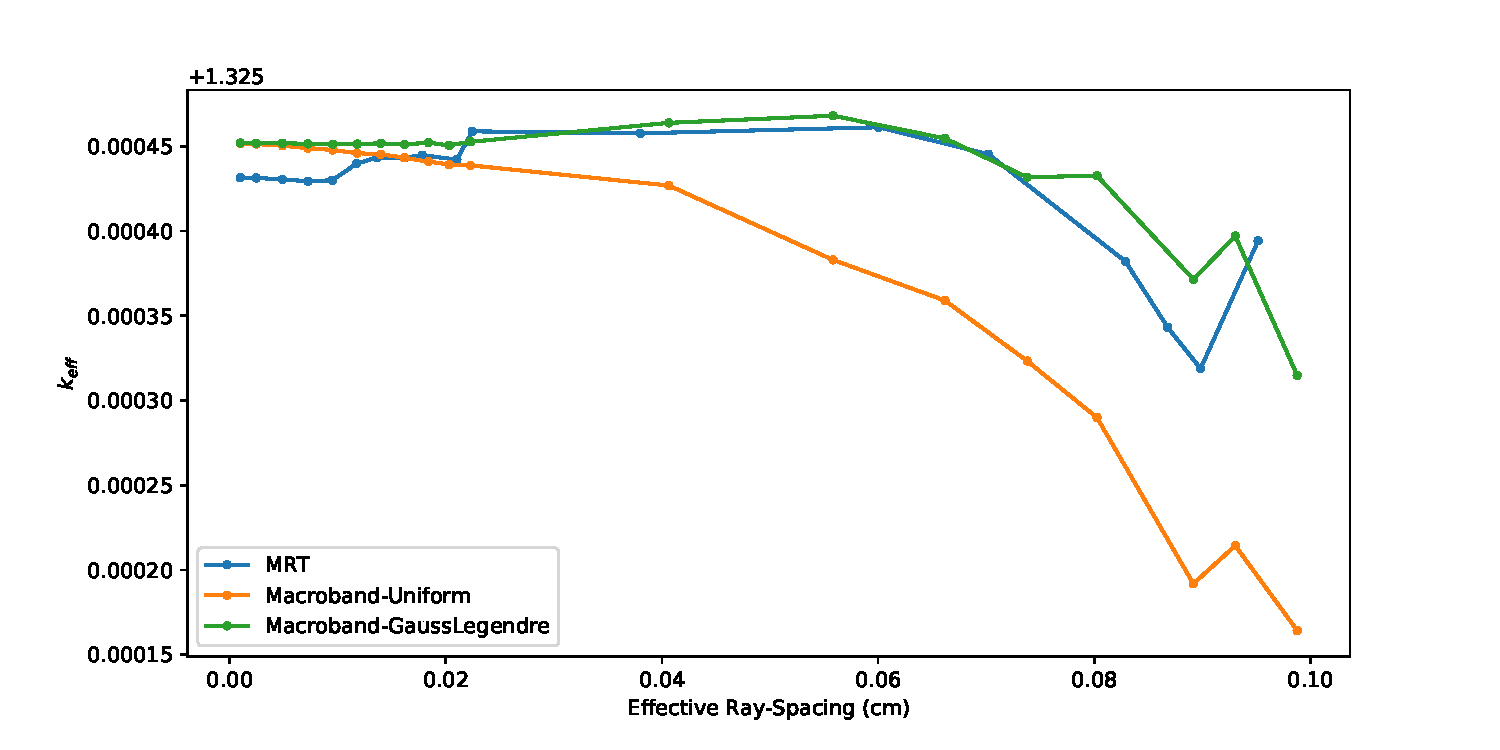
\includegraphics[width=0.65\linewidth]{\figpath/Macroband/EigenvalueComparisons}
            \caption{Eigenvalue comparisons for the different ray-tracing methods over a range of ray-spacings.}
            \label{fig:Results:Macroband:EigenvalueComparisons}
        \end{figure}
        \begin{figure}[h]
            \centering
            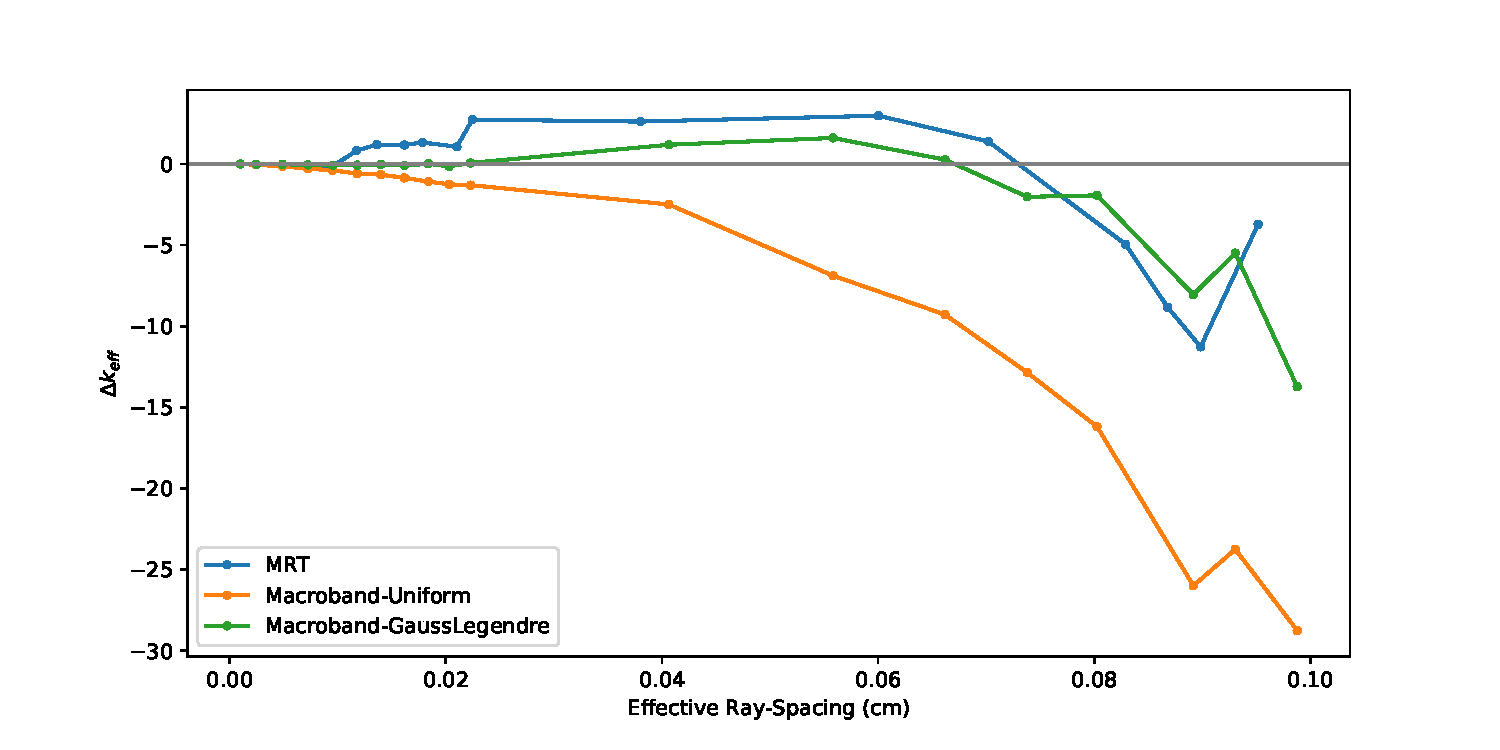
\includegraphics[width=0.65\linewidth]{\figpath/Macroband/EigenvalueError}
            \caption{Eigenvalue errors (relative to finest ray-spacing of that ray-tracing method) for each ray-tracing method over a range of ray-spacings.}
            \label{fig:Results:Macroband:EigenvalueError}
        \end{figure}
        \begin{figure}[h]
            \centering
            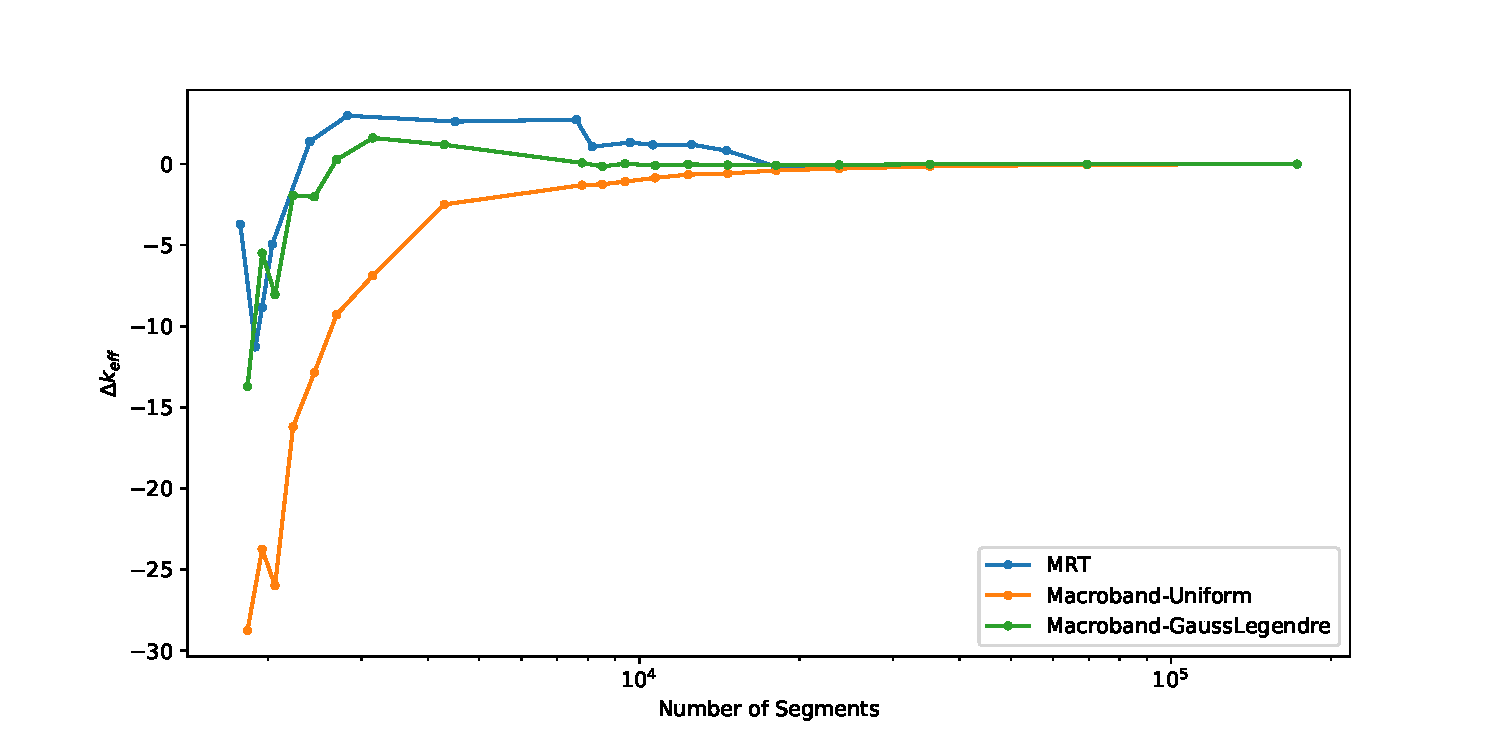
\includegraphics[width=0.65\linewidth]{\figpath/Macroband/ErrorVsNsegs}
            \caption{Eigenvalue errors (relative to finest ray-spacing of that ray-tracing method) for each ray-tracing method as a function of the number of track-segments.}
            \label{fig:Results:Macroband:EigenvalueError vs nsegs}
        \end{figure}

        A visualization of generated rays for this pin-cell are shown in \cref{fig:Results:Macroband:Rays}.
        Each of the macroband methods has obvious ``clustering'' effects near the small surfaces in the computational mesh, this is obvious in the azimuthal divisions in the moderator region outside the pin.
        This clustering is expected, as the macroband method will guarantee rays to pass through these surfaces, unlike the \ac{MRT}.
        Although this may not have significant effect in this case, it may when larger lattice cases are considered, particularly with respect to finely meshed strong absorbers.
        It is also interesting to observe that in the macroband with uniform spacing method, there seem to be concentric patterns where many rays intersect; it may be possible to remove these patterns by using a mobile-chord method within each macroband.

        \begin{figure}[h]
          \centering
          \begin{subfigure}[t]{0.45\linewidth}
            \centering
            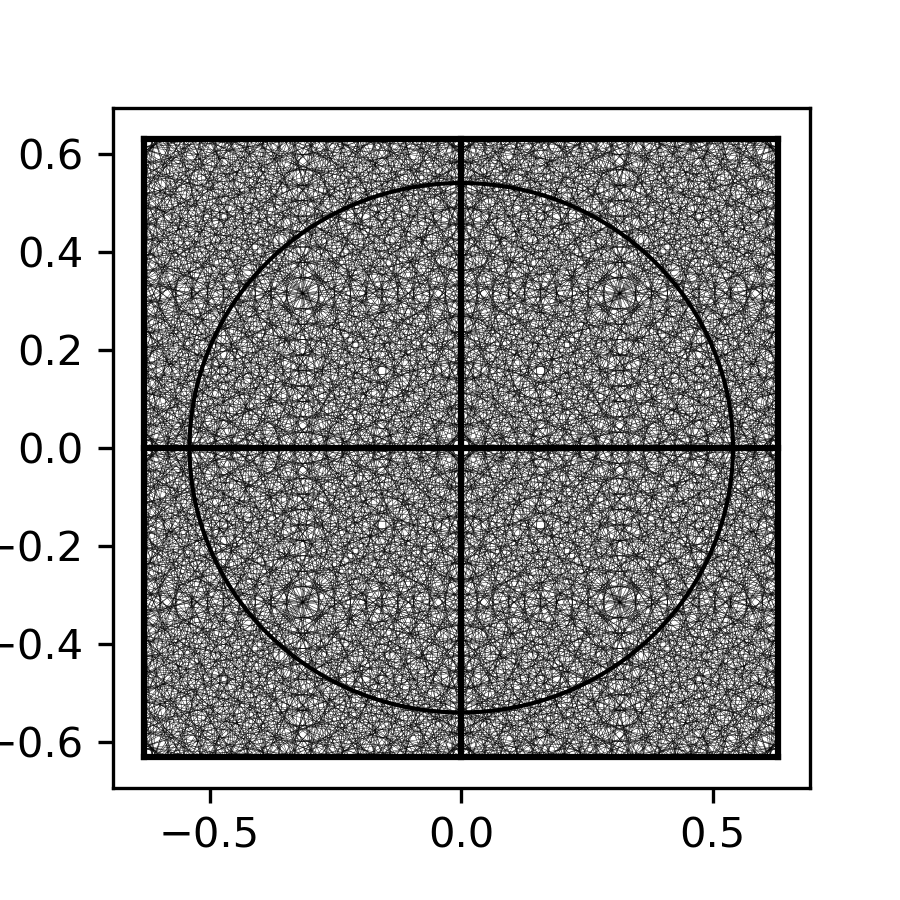
\includegraphics[width=\linewidth]{\figpath/Macroband/MRT_Rays}
            \caption{MRT}
            \label{fig:Results:Macroband:Rays:MRT}
          \end{subfigure}
          \begin{subfigure}[t]{0.45\linewidth}
            \centering
            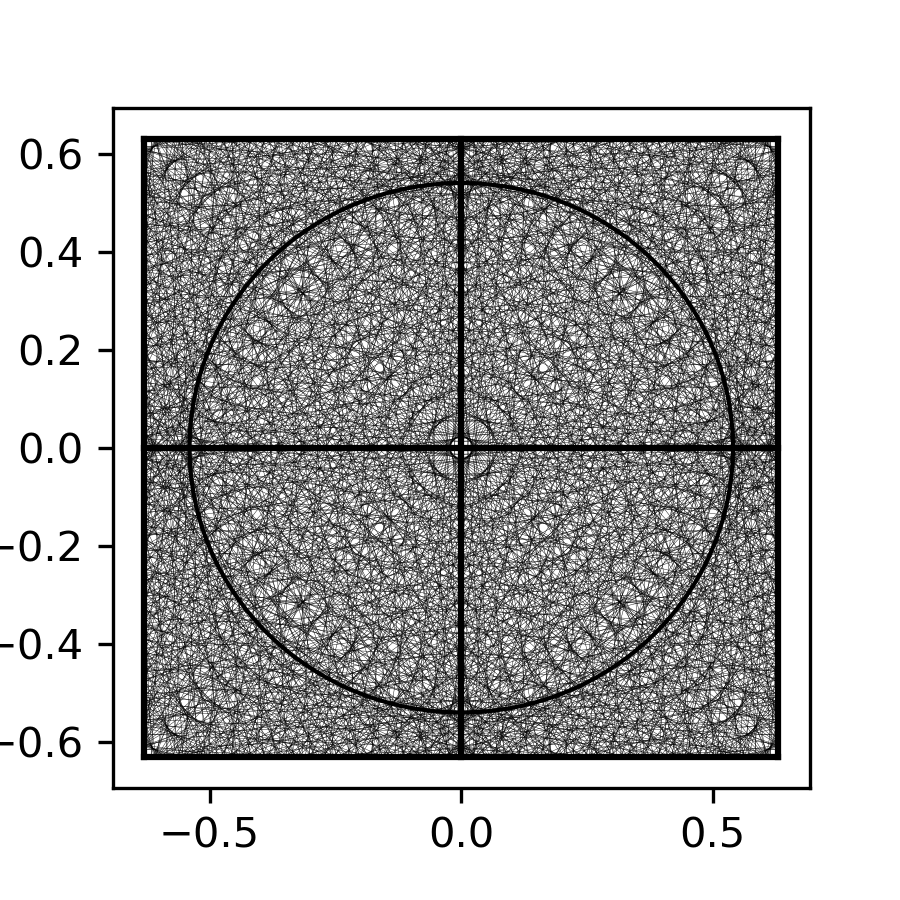
\includegraphics[width=\linewidth]{\figpath/Macroband/MBU_Rays}
            \caption{Macroband-Uniform}
            \label{fig:Results:Macroband:Rays:MBU}
          \end{subfigure}
          \begin{subfigure}[t]{0.45\linewidth}
            \centering
            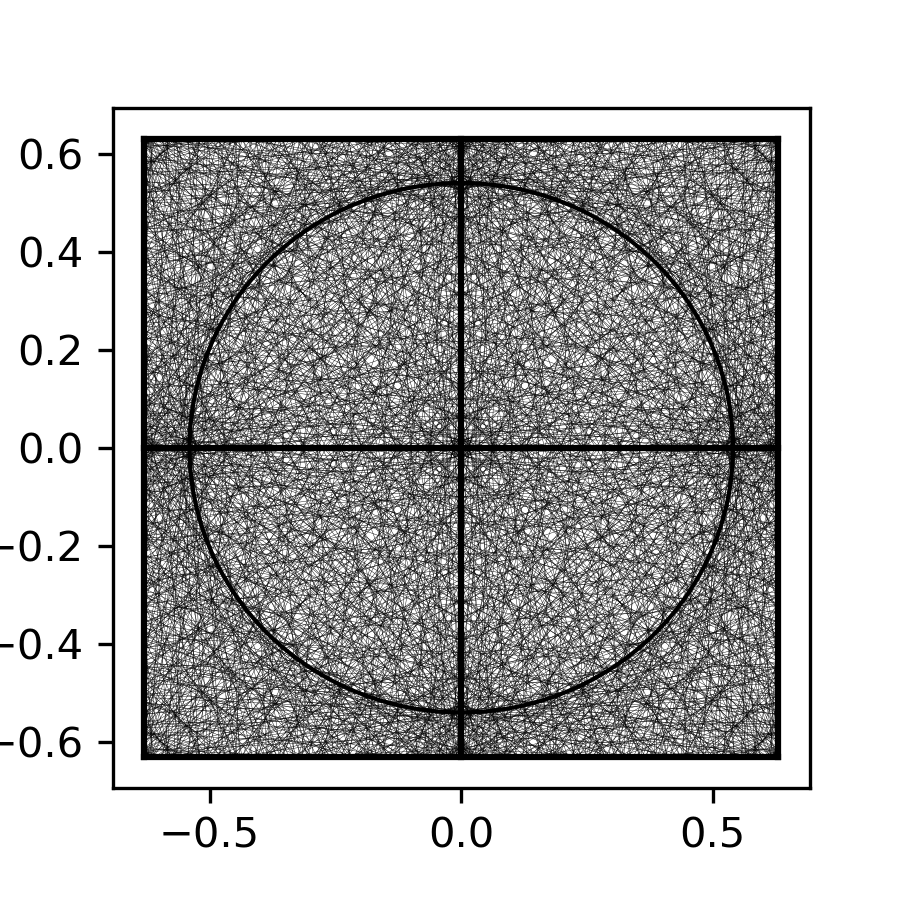
\includegraphics[width=\linewidth]{\figpath/Macroband/MBGL_Rays}
            \caption{Macroband-Gauss-Legendre}
            \label{fig:Results:Macroband:Rays:MBGL}
          \end{subfigure}
          \caption{Visualization of generated rays for an input spacing of 0.05 cm for each ray-tracing method.}
          \label{fig:Results:Macroband:Rays}
        \end{figure}
    }
    %%%%%%%%%%%%%%%%%%%%%%%%%%%%%%%%%%%%%%%%%%%%%%%%%%%%%%%%%%%%%%%%%%%%%%%%%%%%%%
    % Future work
    %%%%%%%%%%%%%%%%%%%%%%%%%%%%%%%%%%%%%%%%%%%%%%%%%%%%%%%%%%%%%%%%%%%%%%%%%%%%%%
    \section{Future work}{\label{sec:Results:Future work}
        The main contributions of this thesis work are the improved \ac{LSMOC}, the macroray ray-tracing techniques, and an improved spatial decomposition scheme, with application toward improving the efficiency of three-dimensional \ac{MOC} calculations.
        Thus far, 2-D studies have been performed on the \ac{LSMOC} with and without multiphysics \cite{Ferrer2016,Fitzgerald2019}, and 3-D studies have been performed without multiphysics \cite{Gunow2018}.
        Future work in this thesis requires larger 2-D multiphysics calculations to be run to verify new default mesh parameters, as well as 3-D multiphysics calculations.

        Work on the spatial decomposition scheme has largely been completed.
        Studies have been performed for 2-D transport calculations, and load-balance has been analyzed for 3-D problems \cite{Fitzgerald2019a}.
        The 2-D transport calculations revealed that some alignment of the spatial domains will have benefits in iteration convergence due to re-entrant flux.
        This indicates that for 3-D calculations, the axially and radially aligned decomposition schemes are likely to have an additional advantage not observed from load-balance results.

        Finally, implementation of the macroray based \ac{MOC} library is currently in progress.
        Several steps are still required for this implementation to be completed: calculations of current for \ac{CMFD} calculations, generalization to 3-D rays, multi-pin calculations, and anisotropic scattering.
        Studies should be performed on two-dimensional transport problems.
        A repetition of the lattice cases run in \cref{sec:Results:2-D Linear Source} should be run with each of the ray-tracing methods in 2-D calculations; this is to verify our treatment of interface conditions, as well as demonstrate the advantage in cases with strong absorbers.
        Additionally, as the methods are extended to three-dimensional problems, a scaling study of ray and segment requirements vs accuracy should be performed on a small problem.
        This study shall require investigation into the effect of directional quadrature modularization.

        An approximate outline of future activities is outlined in \cref{fig:Implementation Plan}.
        \begin{figure}[h]
            \centering
            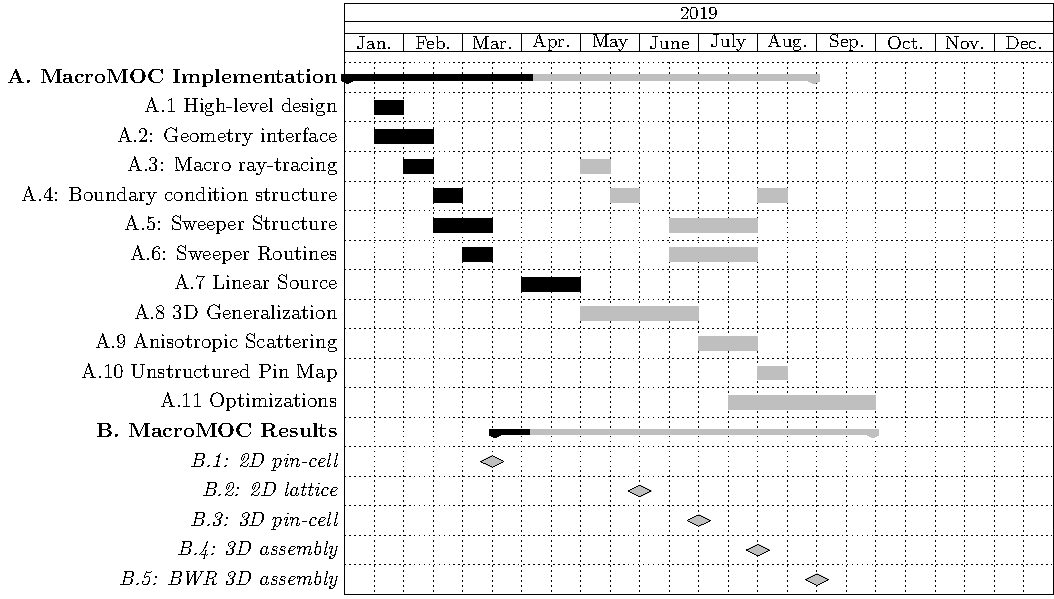
\includegraphics[width=\linewidth]{\figpath/plan/ganttChart.pdf}
            \caption{Possible plan for implementation of macroray \ac{MOC} library.}
            \label{fig:Implementation Plan}
        \end{figure}


    }
    % References
    % \printbibliography
}